% !TeX encoding = utf8
\documentclass[german,aspectratio=169]{beamer}

\usepackage{beamerthemeHM-blue} 
\input{./../../includes/ColorDefinitions}
\input{./../../includes/packages}
\input{./../../includes/meta}
\input{./../../includes/commands}
\input{./../../includes/listing-style}
\lstset{style=ipython}

\graphicspath{{./figs/}}
\setbeamercolor{alerted text}{fg=red}
\title{Recurrent Neural Networks}
\subtitle{}
\author{\href{mailto:zoennchen.benedikt@hm.edu}{\textbf{Benedikt Z\"onnchen}}} 
\date{\today}
%\setdefaultlanguage[spelling=new]{german}

\begin{document}
	
\begin{frame}
	\titlepage
\end{frame}

\section{Motivation}
\begin{frame}
	\frametitle{Motivation}
	\begin{figure}
		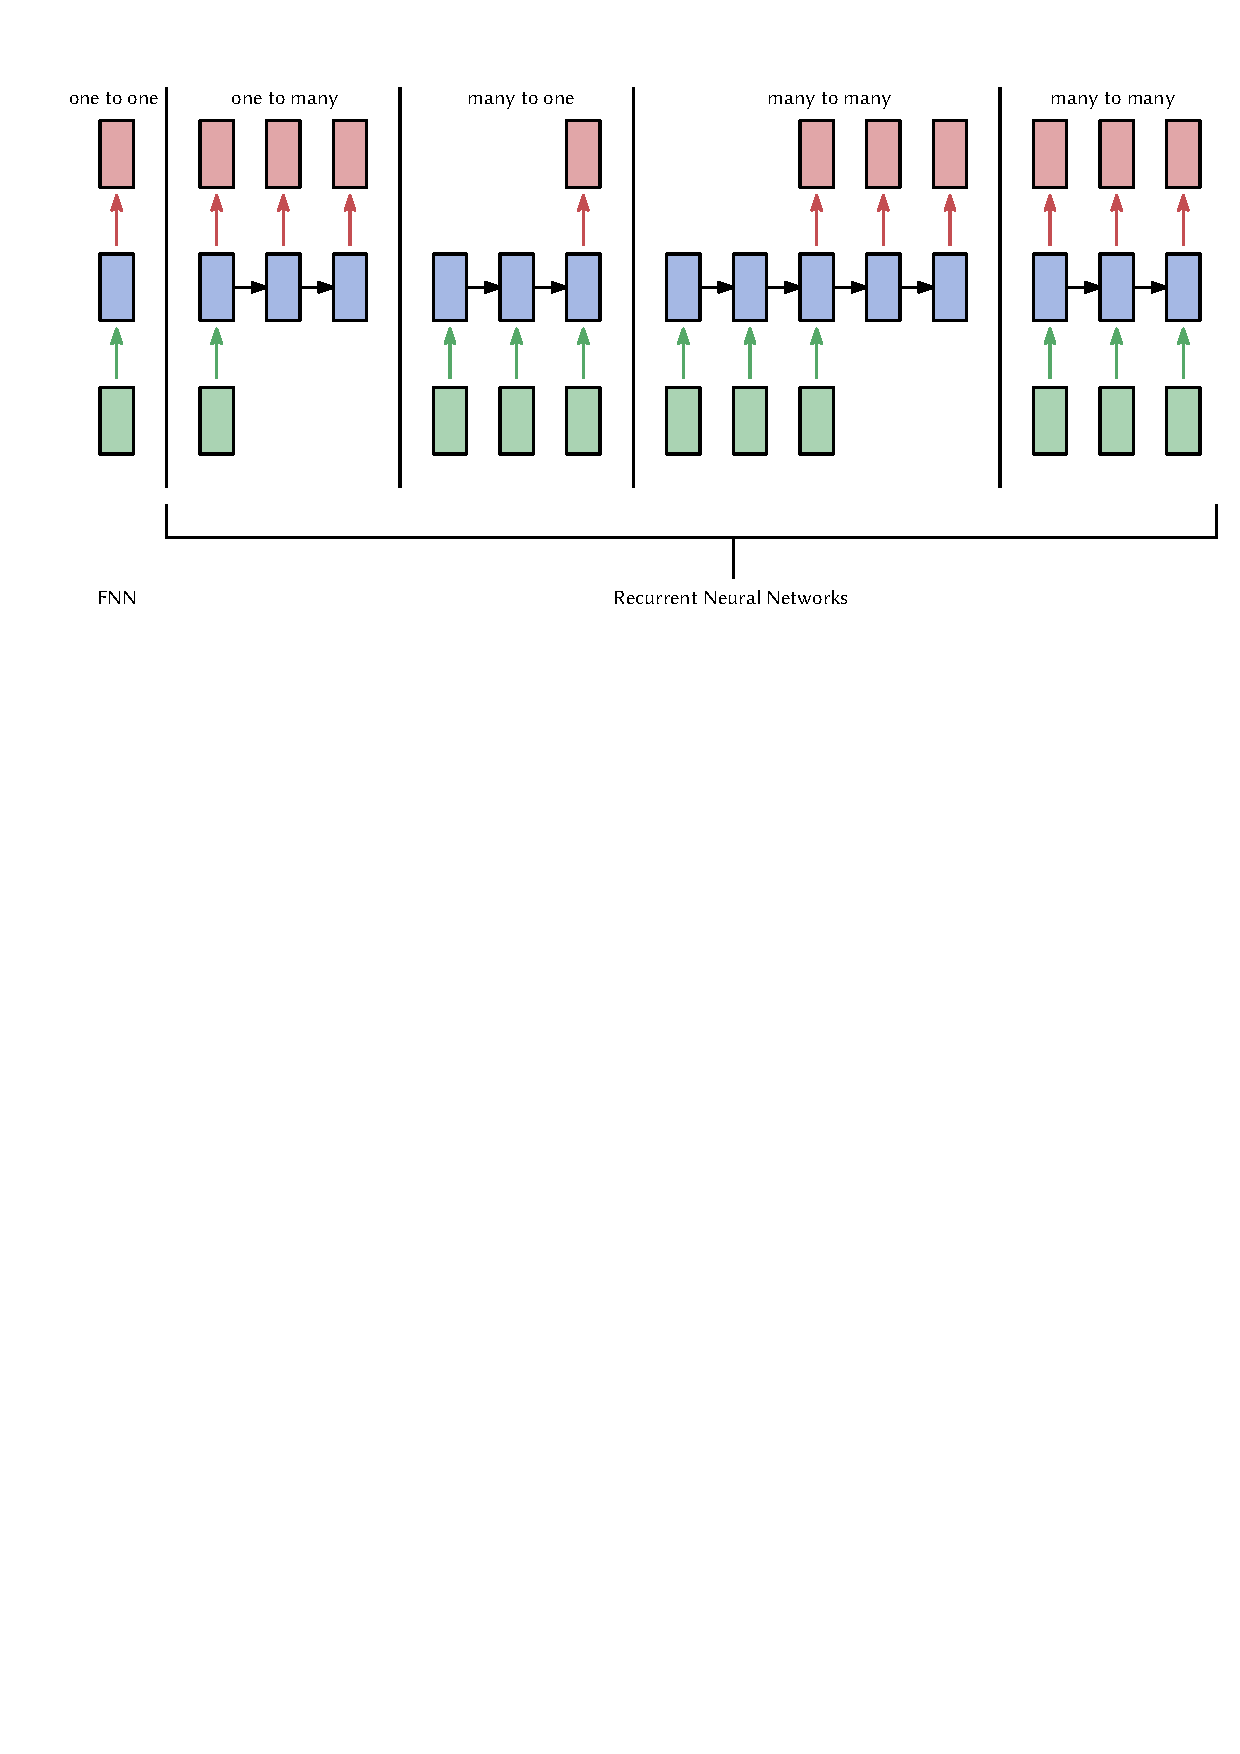
\includegraphics[width=\textwidth]{FNN-vs-RNN}
	\end{figure}
\end{frame}


\section{Von Feedforward zu Recurrent}
\begin{frame}
	\frametitle{Von Feedforward zu Recurrent}
	Die Eingabe durchläuft im Falle von \term{Feedforward Neuronale Networks} das Netz von vorne nach hinten ohne Zyklus.
	Das Netz bildet einen gerichteten azyklischen Graphen.
\end{frame}


\begin{frame}
	\frametitle{Von Feedforward zu Recurrent}
	
	\begin{figure}
		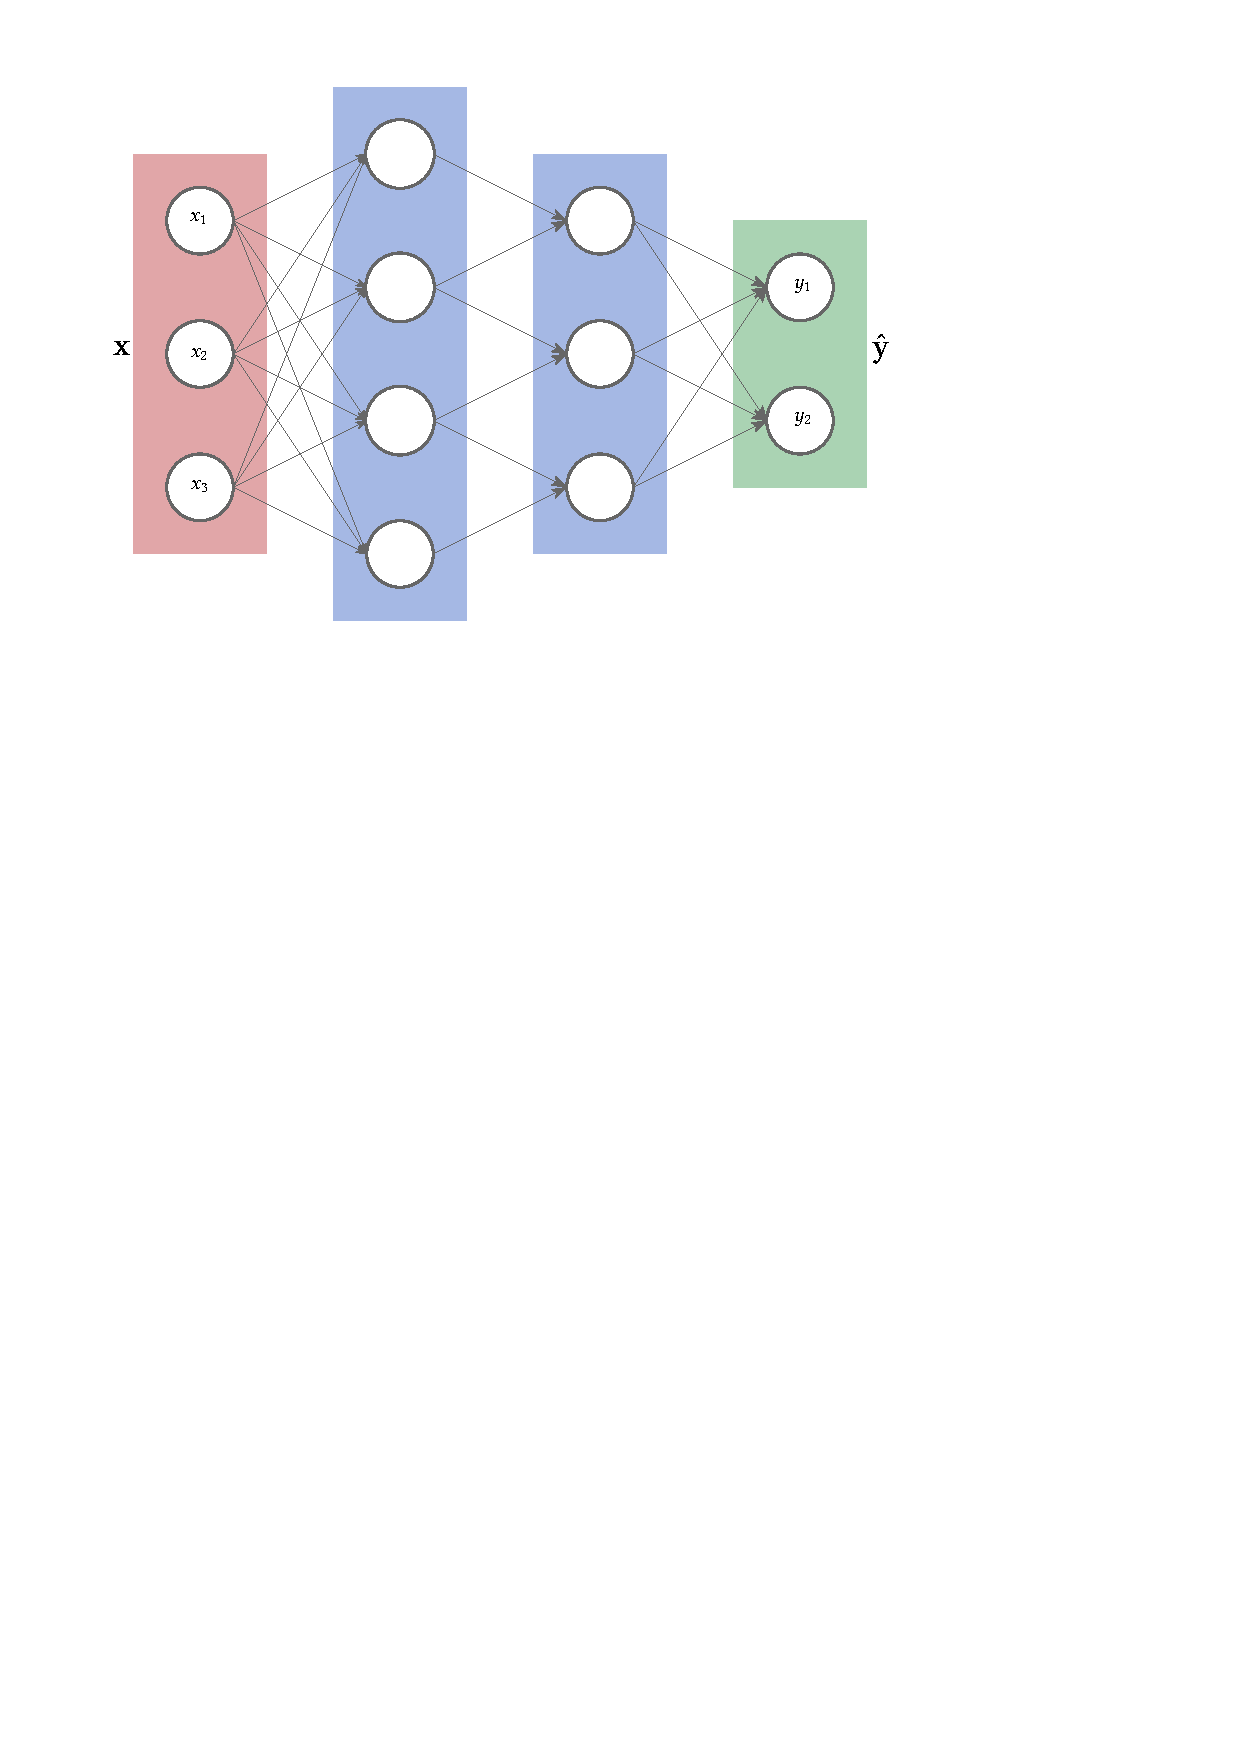
\includegraphics[width=0.7\textwidth]{fnn.pdf}
	\end{figure}
	
\end{frame}

\begin{frame}
	\frametitle{Von Feedforward zu Recurrent}
	Führen wir Zyklen in das Netz ein, sprechen wir von einem sog. \term{Recurrent Neural Network (RNN)}.
\end{frame}

\begin{frame}
	\frametitle{Von Feedforward zu Recurrent}
	\begin{figure}
		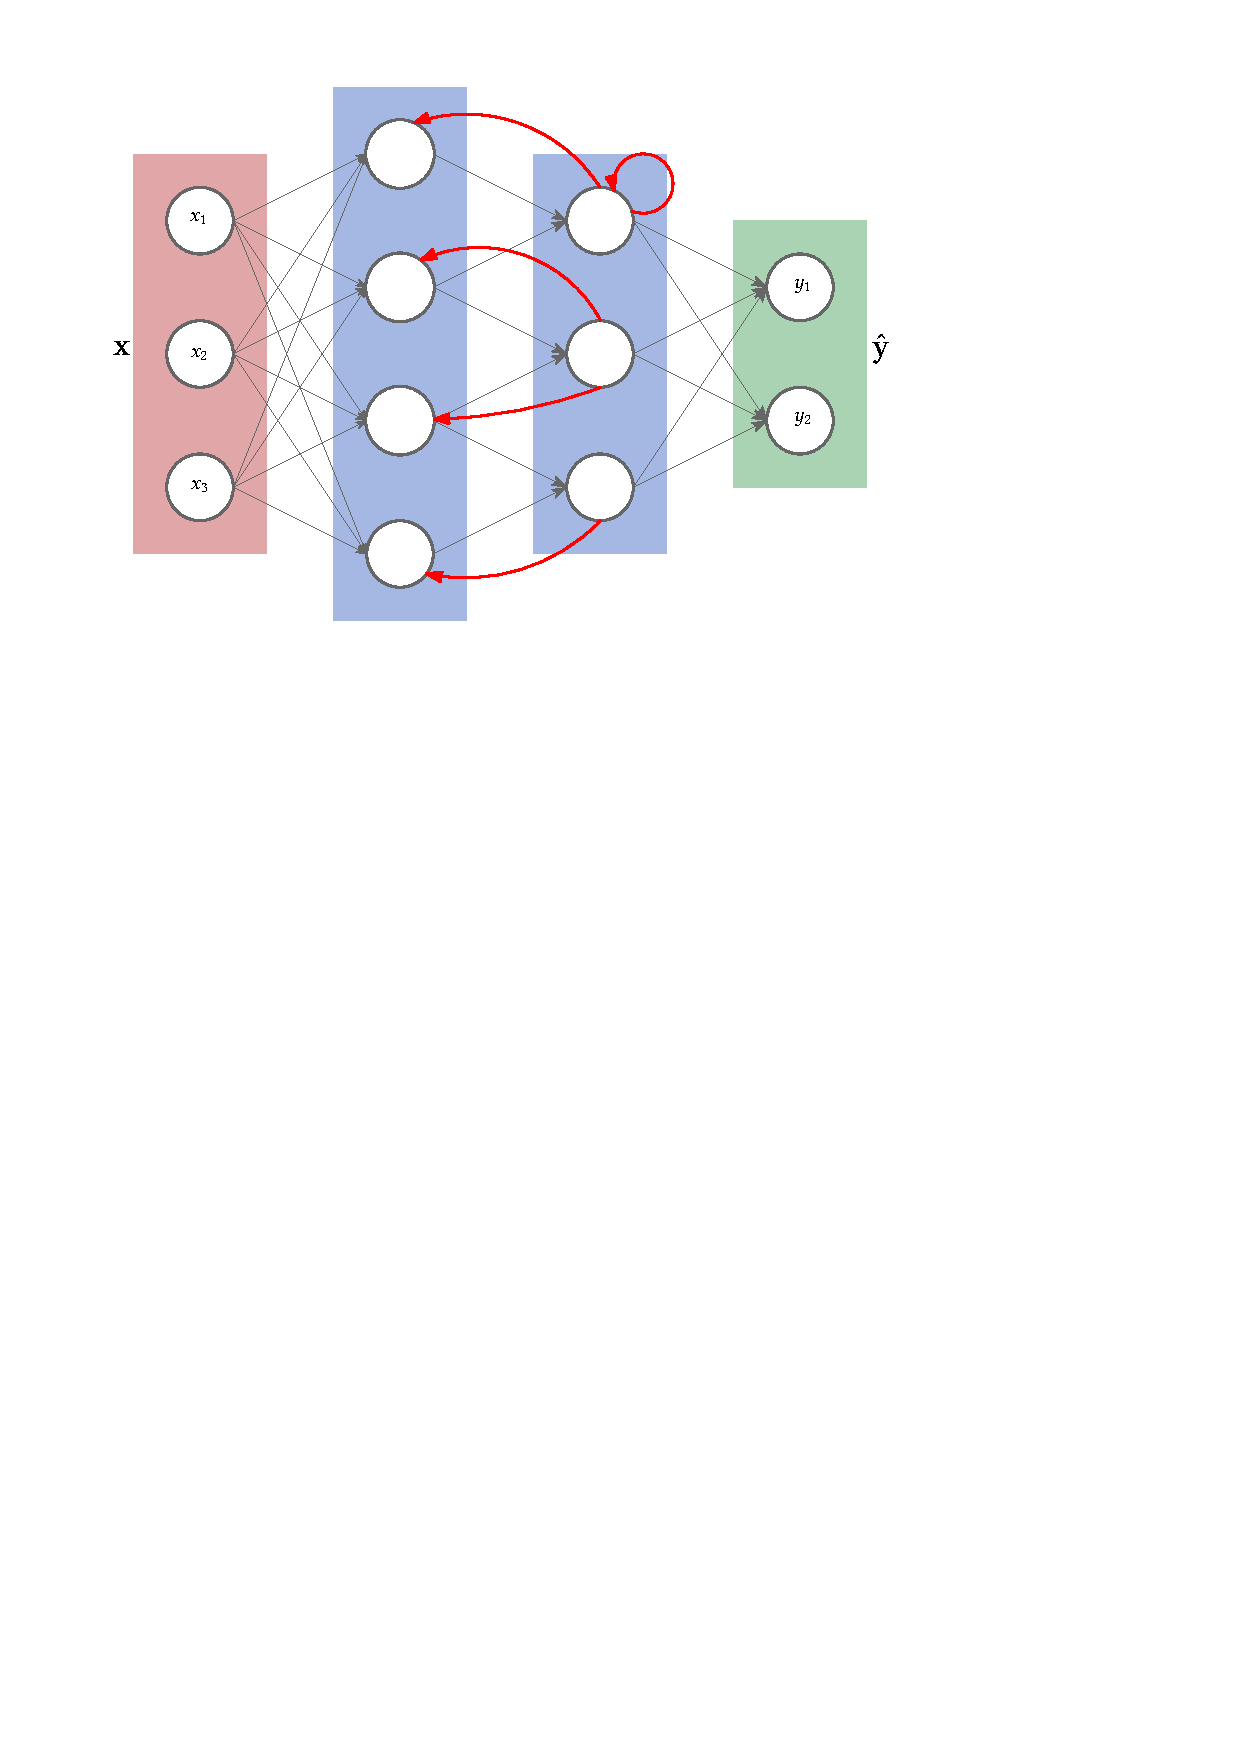
\includegraphics[width=0.7\textwidth]{rnn}
	\end{figure}
\end{frame}


\begin{frame}
	\frametitle{Von Feedforward zu Recurrent}
	\framesubtitle{Hopfield Networks}
	\begin{columns}
		\begin{column}{0.6\textwidth}
			\begin{enumerate}[label=$\bullet$]
				\item Erste Einführung durch John J. Hopfield \cite{Hopfield1982} im Jahr 1982
				\item Motiviert durch:
					\begin{enumerate}[label=$\circ$]
						\item Automatische Fehlerkorrektur
						\item Informationsvervollständigung
						\item Dynamische Systeme mit stabilen Zuständen (Beispiel: Planetensysteme)
					\end{enumerate}
				\item Fehlerhafte oder unvollständige Information 'konvergiert' zu korrekter Information (Assoziation)
			\end{enumerate}
		\end{column}
		\begin{column}{0.3\textwidth}
			\begin{figure}
				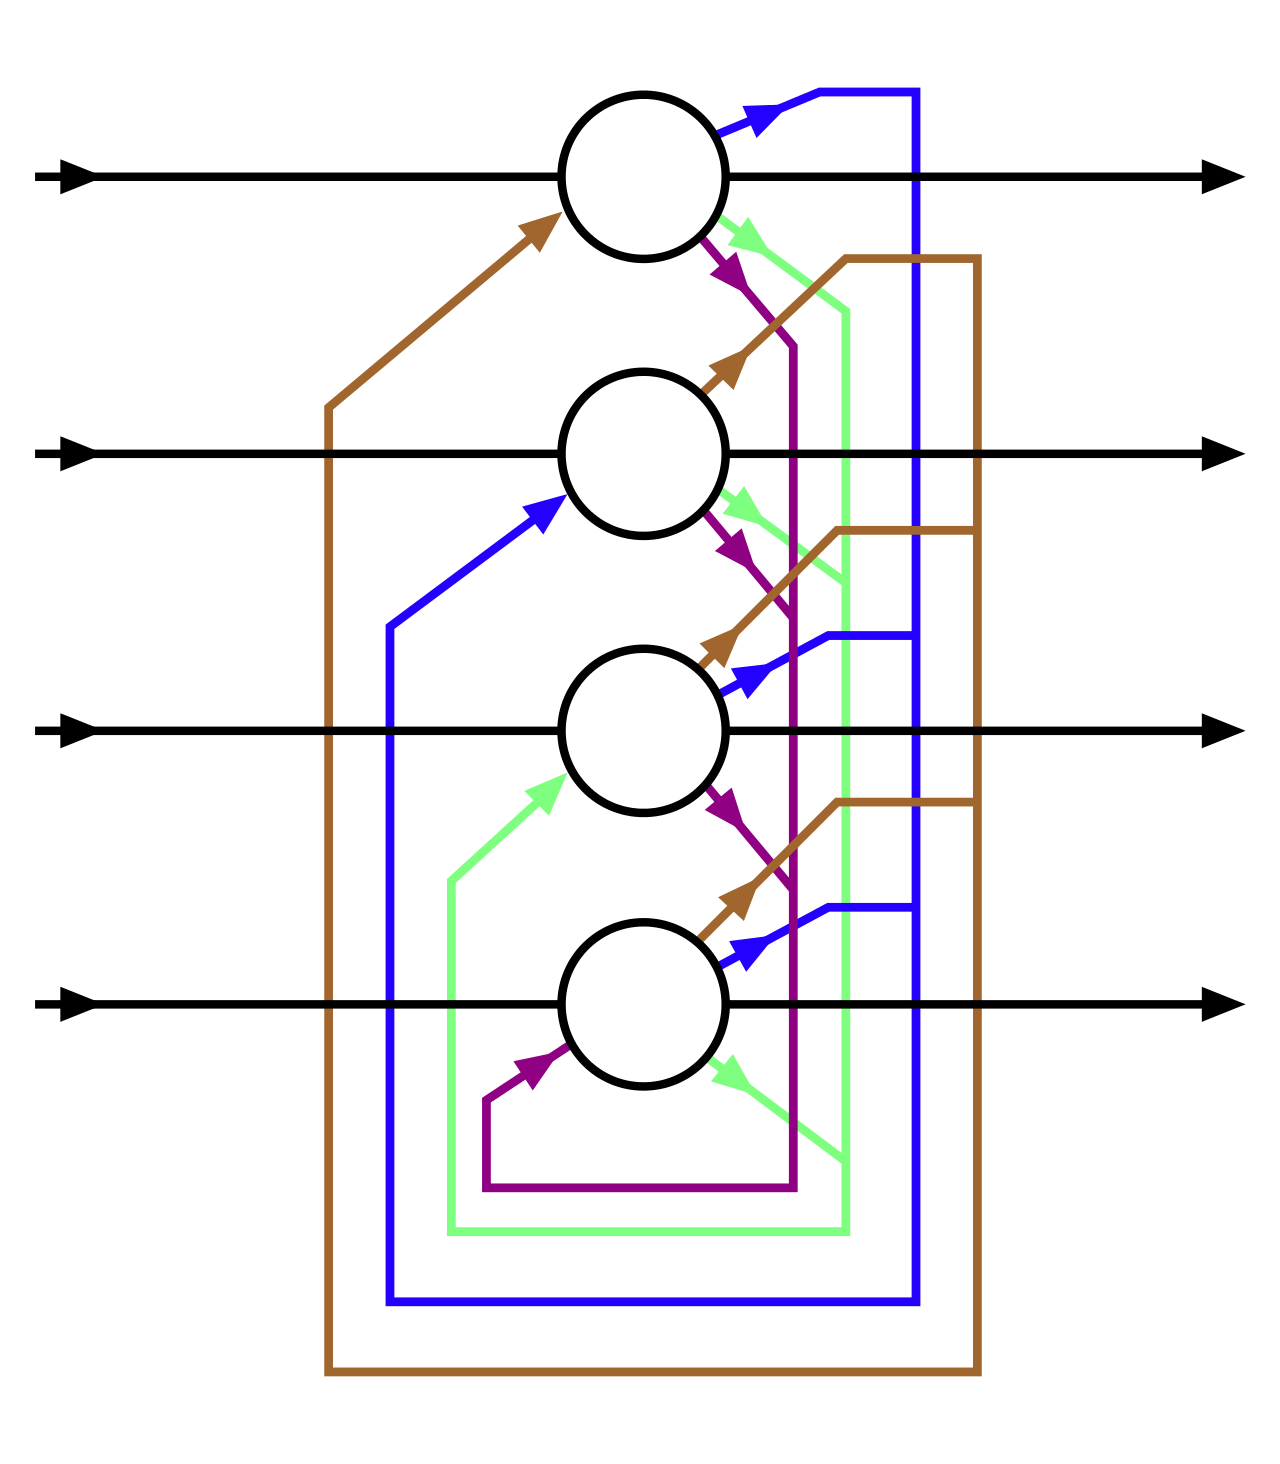
\includegraphics[width=\textwidth]{hopfield-net.png}
			\end{figure}
		\end{column}
	\end{columns}
\end{frame}

\begin{frame}
	\frametitle{Von Feedforward zu Recurrent}
	\framesubtitle{Hopfield Networks am Beispiel der Platzwahl}
	\begin{figure}
	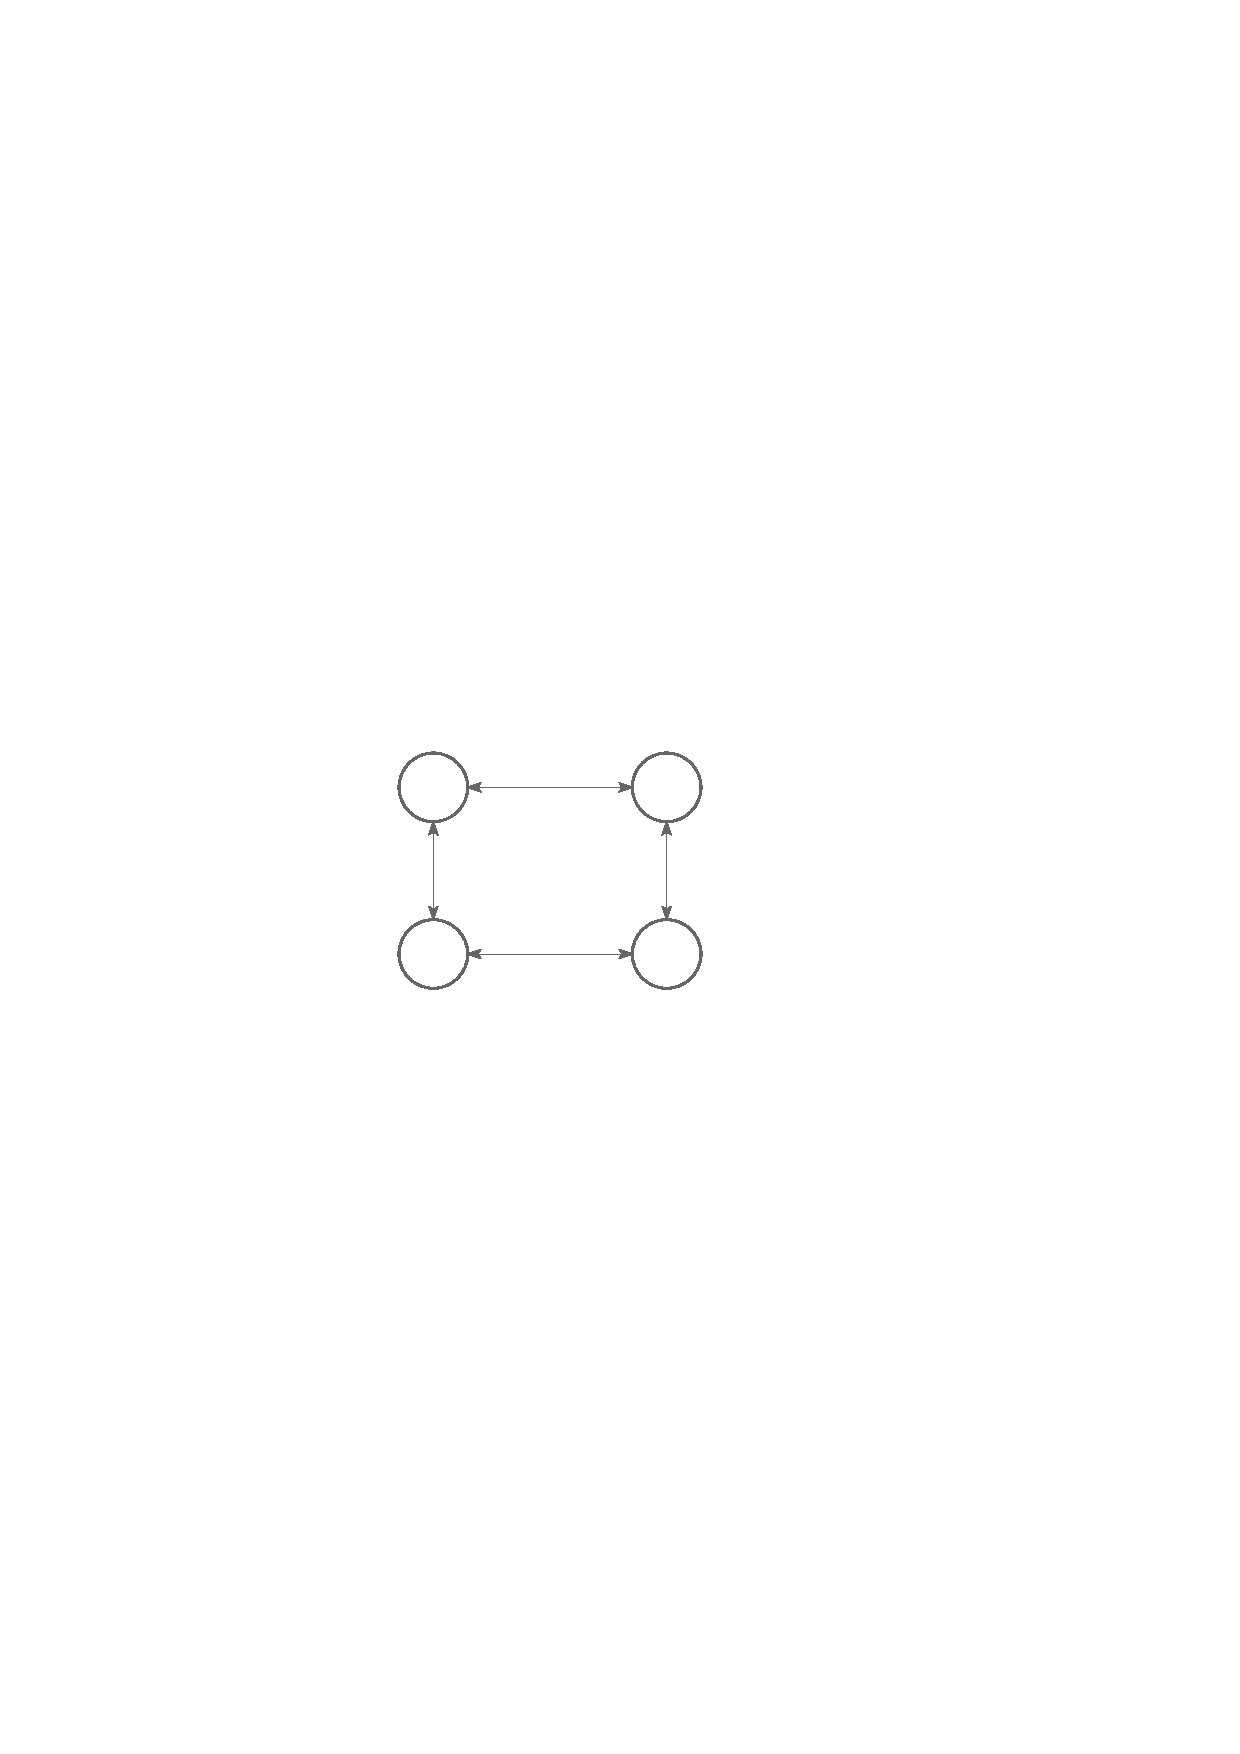
\includegraphics[width=0.5\textwidth]{desk-example}
	\end{figure}
\end{frame}

\begin{frame}
	\frametitle{Von Feedforward zu Recurrent}
	\begin{columns}
		\begin{column}{0.3\textwidth}
			\begin{enumerate}[label=$\bullet$]
				\item Eingabe: Sequenz $\mathbf{X} = \xx_0, \ldots, \xx_n$
				\item Ausgabe: Sequenz: $\mathbf{Y} = \yy_0, \ldots, \yy_n$
				\item Hidden States: $\mathbf{H} = \mathbf{h}_0, \ldots, \mathbf{h}_n$
			\end{enumerate}
		\end{column}
		\begin{column}{0.7\textwidth}
			\begin{figure}
				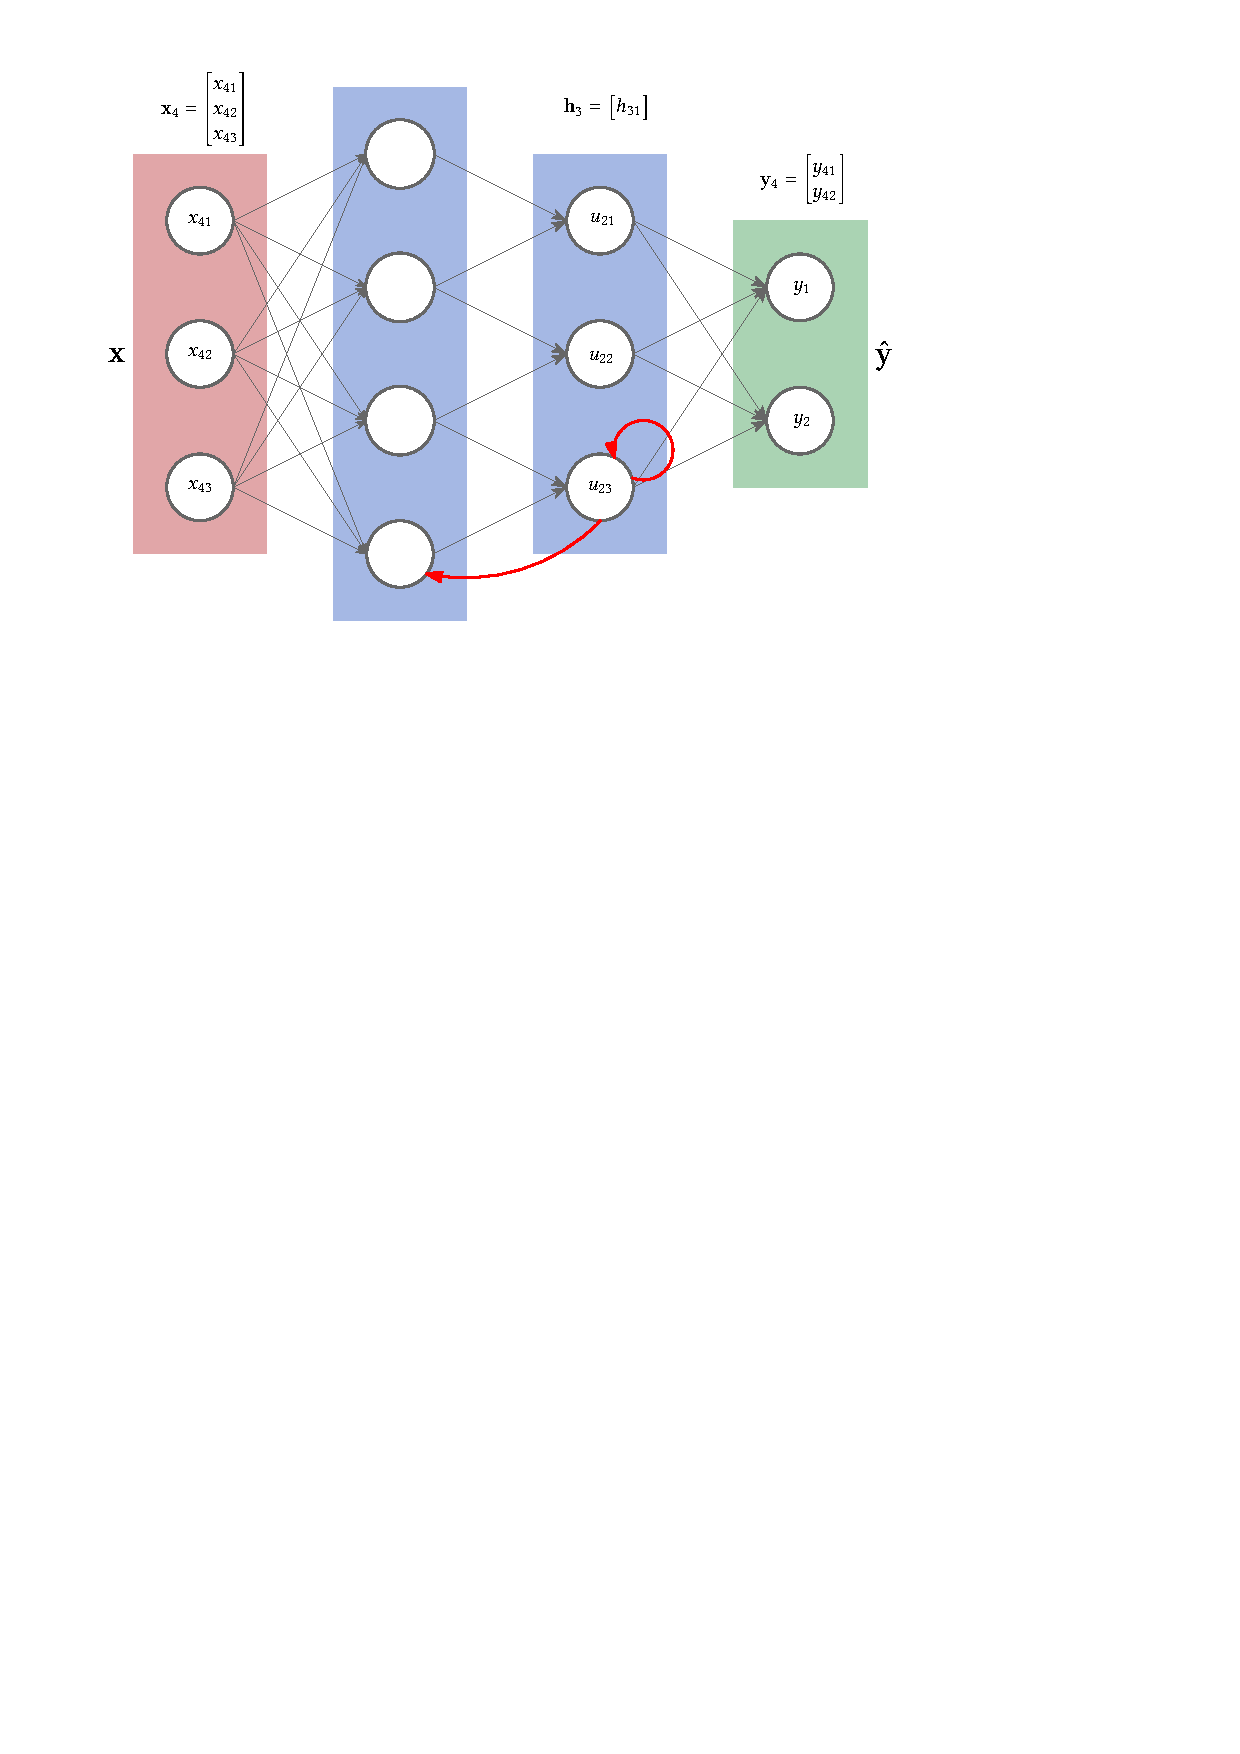
\includegraphics[width=\textwidth]{rnn-labeled}
			\end{figure}
		\end{column}
	\end{columns}
\end{frame}


\begin{frame}
	\frametitle{Von Feedforward zu Recurrent}
	\begin{columns}
		\begin{column}{0.35\textwidth}
			\begin{enumerate}[label=$\bullet$]
				\item Eingabe: Sequenz $\mathbf{X} = \xx_0, \ldots, \xx_n$
				\item Ausgabe: Sequenz: $\mathbf{Y} = \yy_0, \ldots, \yy_n$
				\item Hidden States: $\mathbf{H} = \mathbf{h}_0, \ldots, \mathbf{h}_n$
			\end{enumerate}
		\end{column}
		\begin{column}{0.65\textwidth}
			\begin{figure}
				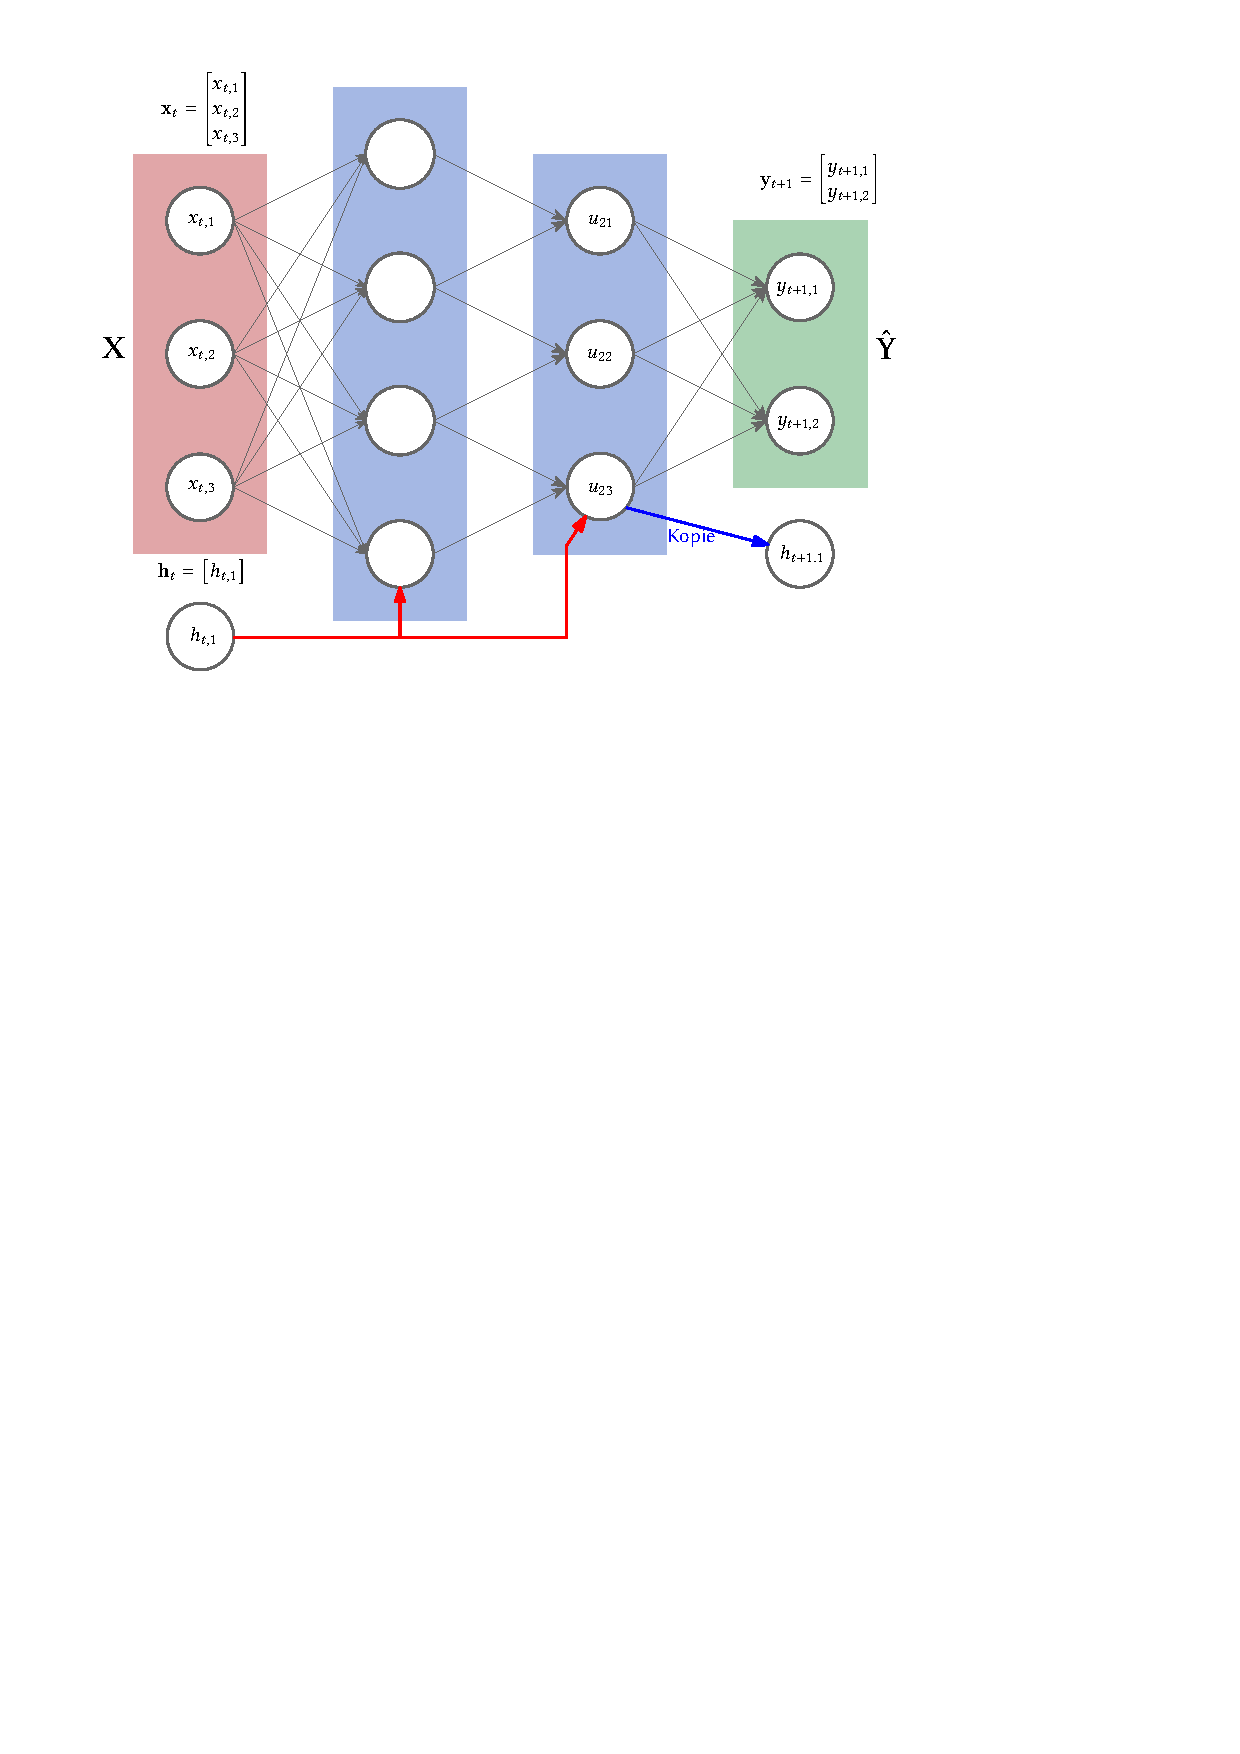
\includegraphics[width=\textwidth]{rnn-labeled-unfold}
			\end{figure}
		\end{column}
	\end{columns}
\end{frame}

\begin{frame}
	\frametitle{Von Feedforward zu Recurrent}
\begin{columns}
	\begin{column}{0.3\textwidth}
	\begin{figure}
		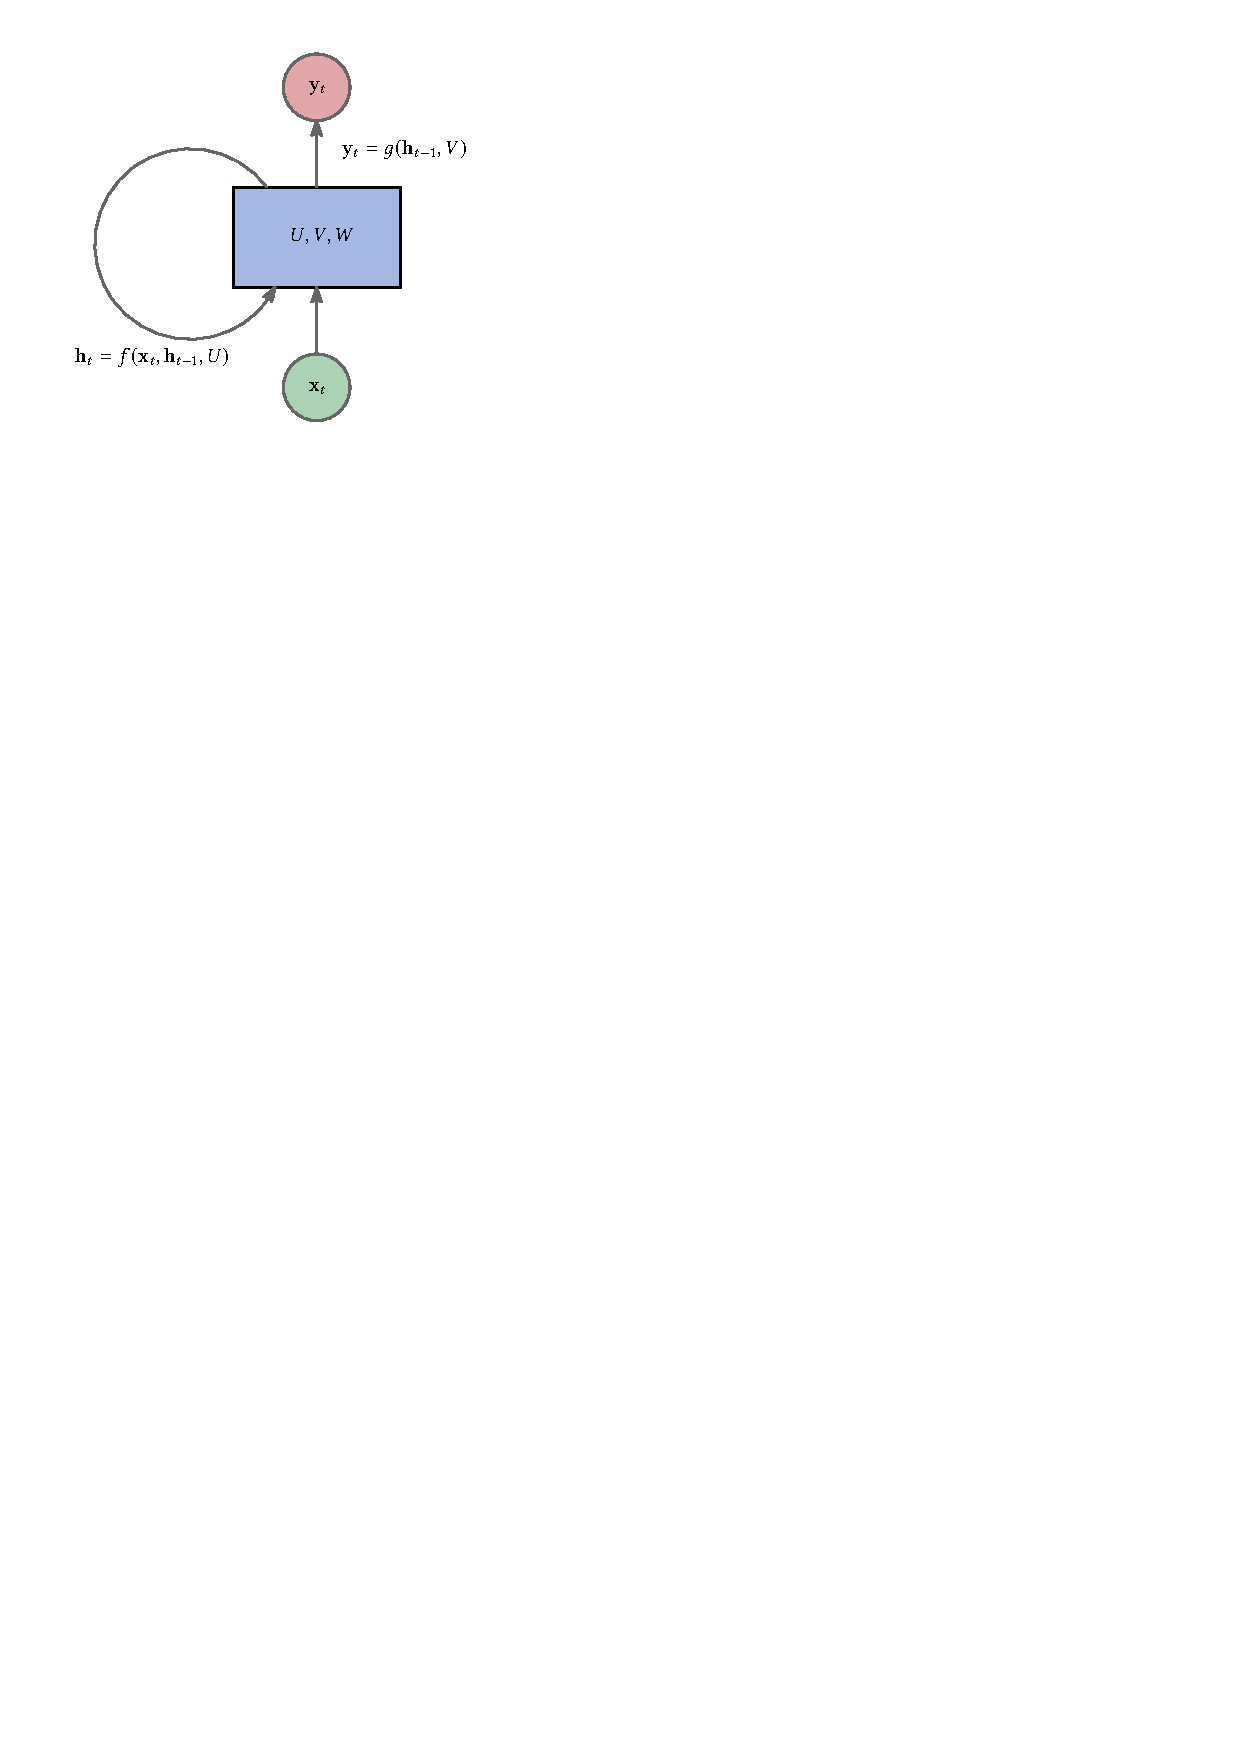
\includegraphics[scale=0.7]{rnn-diagram.pdf}
	\end{figure}
	\end{column}
	\hfill
	\begin{column}{0.7\textwidth}
		\begin{figure}
			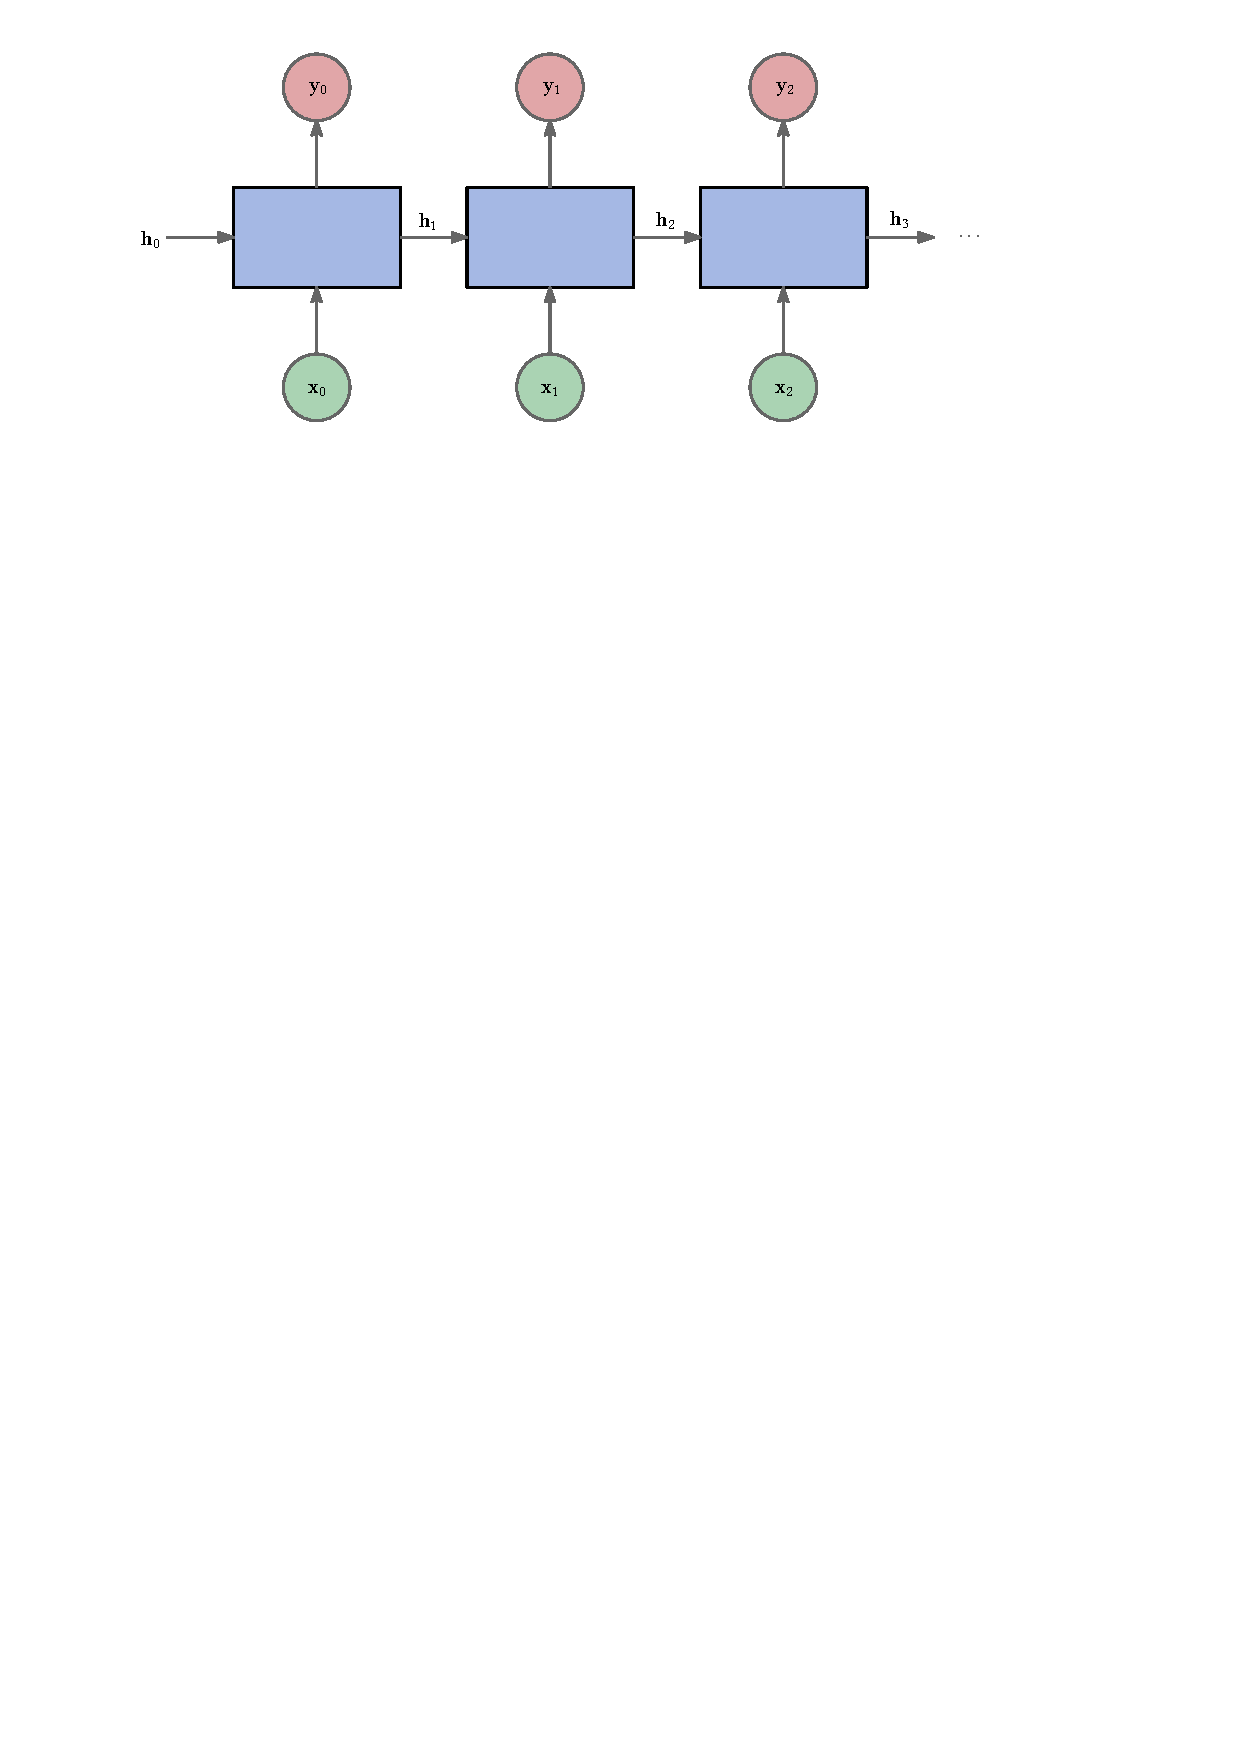
\includegraphics[scale=0.7]{rnn-diagram-unfold}
		\end{figure}
	\end{column}
\end{columns}
\end{frame}


\begin{frame}
	\frametitle{Von Feedforward zu Recurrent}
	\begin{theorem}
		Für jedes \term{RNN} gibt es ein \term{Feedforward Network} mit dem gleichen Verhalten über eine endliche Zeit \cite{Rumelhart1987}.
	\end{theorem}
	\begin{figure}
		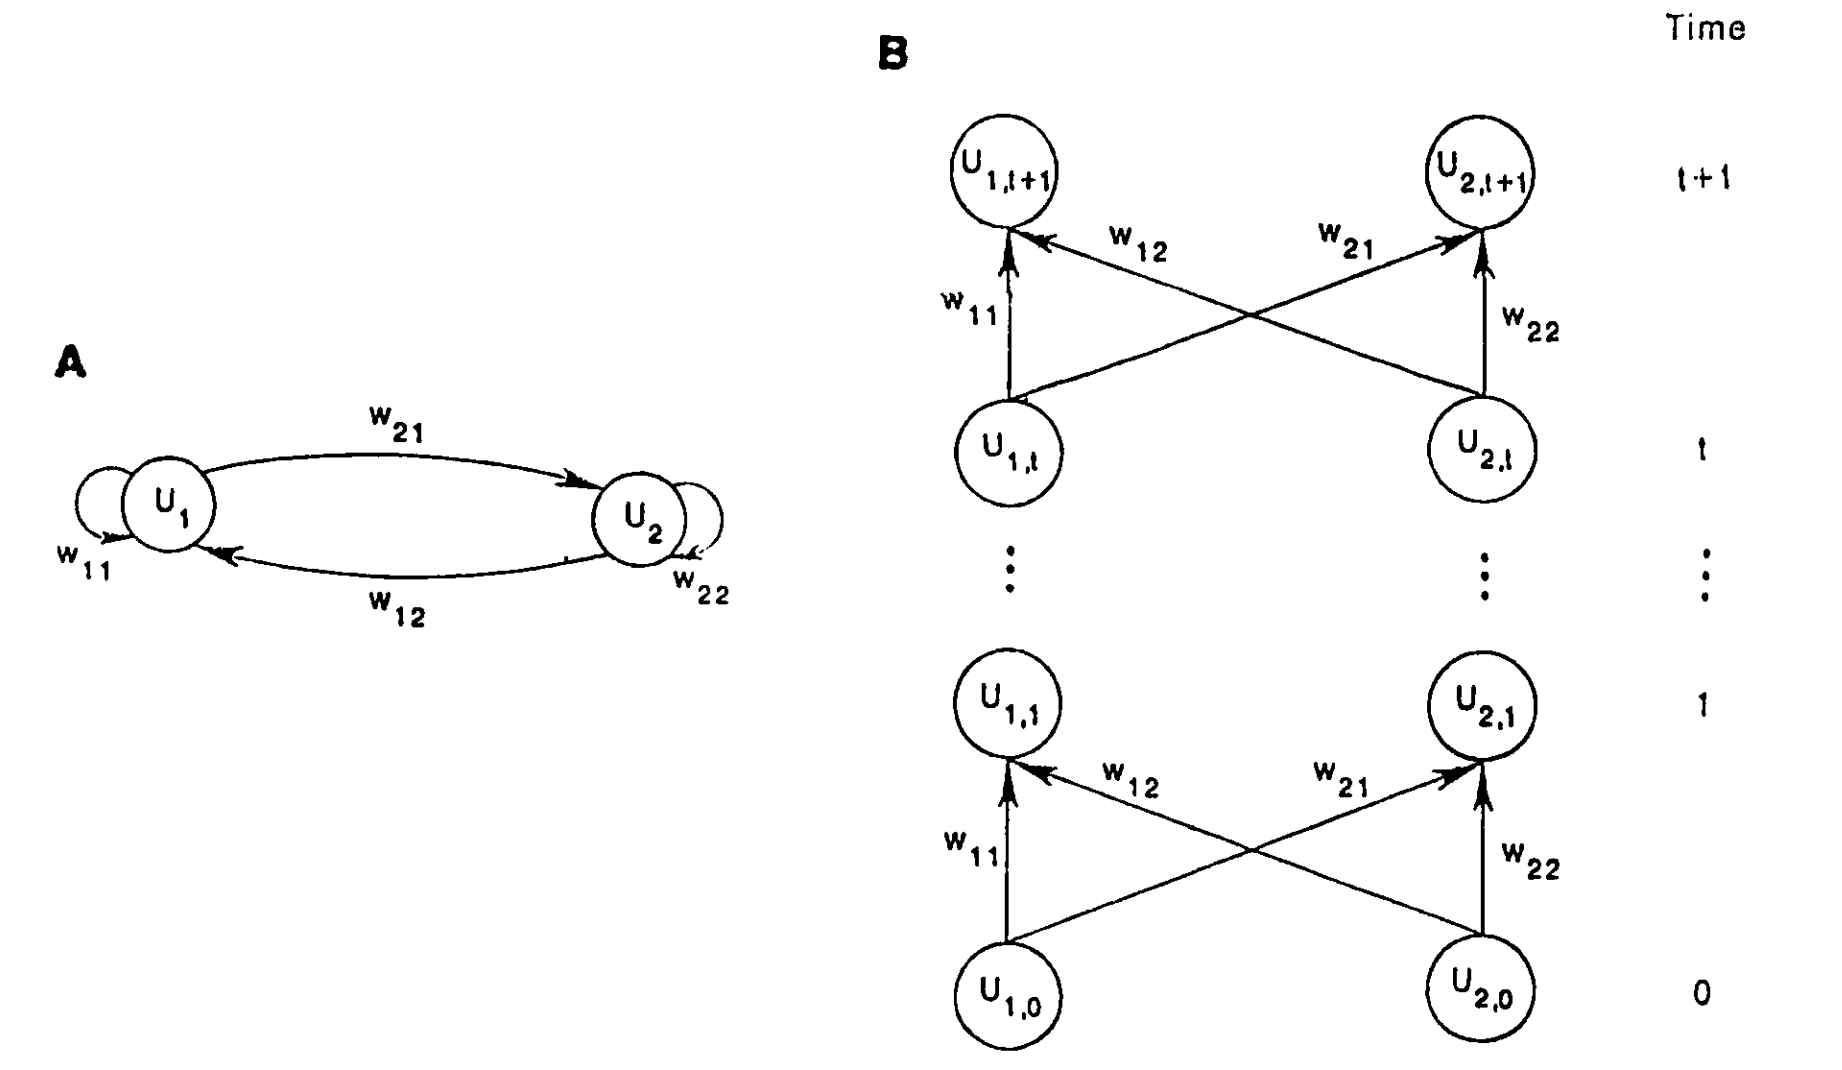
\includegraphics[width=0.55\textwidth]{simplest-rnn}
	\end{figure}
\end{frame}

\begin{frame}
	\frametitle{Recurrent Neural Networks}
	\framesubtitle{Training (Gradient Descent)}
	\hl{Probleme}:
	\begin{enumerate}[label=$\bullet$]
		\item Black Box Problem
		\item Berechnungsaufwand (besonders beim Training) $\Rightarrow$ hoher Ressourcenverbrauch
		\item Je komplexer das Netz desto mehr Daten werden fürs Training gebraucht
		\item Keine Garantie für Korrektheit
		\item Explodierende oder verschwindende Gradienten
		\item Information tendiert sich ``auszuwaschen''
		\item Schlechtes Langzeitgedächtnis
	\end{enumerate}
\end{frame}

%\begin{frame}
%	\frametitle{Recurrent Neural Networks}
%	\framesubtitle{Training: Backpropagation trough time BPTT}
%	Wir haben Antworten: $(x_1, y_1) = (0,0)$ und $(x_2, y_2) = (1,1)$. Initialisiere Parameter zufällig, z.B.: $w_0 = 3, w_1 = 6$
%	\begin{equation*}
%		h_\theta(x) = \underbrace{3}_{w_0} x + \underbrace{6}_{w_1}
%	\end{equation*}
%	Daraus ergeben sich Fehler:
%	\begin{equation*}
%		\begin{split}
%			y_1 - h_\theta(x_1) = y_1 - h_\theta(0) = 0 - 6 = -6\\
%			y_2 - h_\theta(x_2) = y_2 - h_\theta(1) = 1 - 9 = -8
%		\end{split}
%	\end{equation*}
%	
%	Wir suchen die \term{Parameter} $\theta$, sodass der Fehler (oder auch die \term{Kostenfunktion})
%	\begin{equation*}
%		J(\theta) = (y_1 - h_\theta(x_1))^2 + (y_1 - h_\theta(x_2))^2
%	\end{equation*}
%	minimal wird!
%\end{frame}

%\begin{frame}
%	\frametitle{Von Feedforward zu Recurrent}
%	\framesubtitle{Hopfield Networks am Beispiel der Platzwahl}
%	\begin{quoting}
%		``In general, the procedure for a recurrent network is that an input (generally a sequence) is
%		presented to the system while it runs for some number of iterations. At certain specified times
%		during the operation of the system, the output of certain units are compared to the target for
%		that unit at that time and error signals are generated. Each such error signal is then passed
%		back through the network for a number of iterations equal to the number of iterations used in
%		the forward pass.''  \cite{Rumelhart1987}
%	\end{quoting}
%\end{frame}

\begin{frame}[allowframebreaks]
	\frametitle{Referenzen}
	{\scriptsize% dirty fix for the non-chapter bib
		\bibliographystyle{apalike}
		\bibliography{./../../literature/references.bib}}
\end{frame}

\end{document}